\subsection{Предел $\lim_{x\to 0} \frac{\sin x}{x}$.}

\[ \lim_{x \to 0} \frac{\sin x}{x} = 1 \]

\begin{tcolorbox}[title=Доказательство, breakable]
    Рассмотрим случай, когда $x \to 0+0$ (т.е. $0 < x < \frac{\pi}{2}$).
    
    \begin{center}
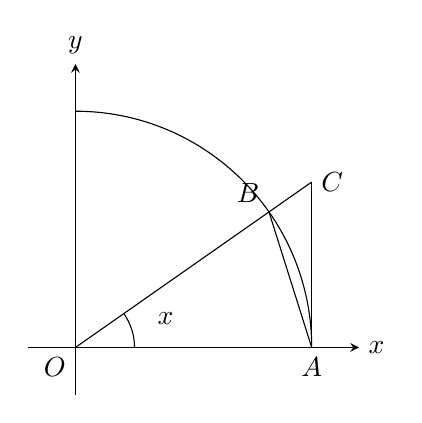
\begin{tikzpicture}[scale=3]
    % Настройки
    \def\ang{35} % Угол x (можно менять, 35 градусов выглядит наглядно)

    % Координаты
    \coordinate (O) at (0,0);
    \coordinate (A) at (1,0);
    \coordinate (B) at (\ang:1);          % Точка на окружности
    \coordinate (C) at (1, {tan(\ang)});  % Точка на касательной

    % Оси координат
    \draw[->, >=stealth] (-0.2,0) -- (1.2,0) node[right] {$x$};
    \draw[->, >=stealth] (0,-0.2) -- (0,1.2) node[above] {$y$};

    % Единичная окружность (дуга 90 градусов)
    \draw (1,0) arc (0:90:1);

    % Основные линии фигуры
    \draw (O) -- (C);       % Гипотенуза большого треугольника (секущая)
    \draw (A) -- (C);       % Касательная (тангенс)
    \draw (A) -- (B);       % Хорда

    % Обозначение угла x
    \draw (0.25,0) arc (0:\ang:0.25);
    \node at (\ang/2:0.4) {$x$};

    % Подписи точек
    \node[below left] at (O) {$O$};
    \node[below] at (A) {$A$};
    \node[above left] at (B) {$B$};
    \node[right] at (C) {$C$};

\end{tikzpicture}
\end{center}

    Рассмотрим единичную окружность ($R=1$). Угол $x$ измеряется в радианах.
    Сравним площади трех фигур:
    \begin{enumerate}
        \item \textbf{Треугольник $\triangle OAB$:} (вписанный)
        \[ S_{\triangle OAB} = \frac{1}{2} R^2 \sin x = \frac{1}{2} \sin x \]
        \item \textbf{Круговой сектор $OAB$:}
        \[ S_{\text{сект}} = \frac{1}{2} R^2 x = \frac{1}{2} x \]
        \item \textbf{Треугольник $\triangle OAC$:} (описанный, прямоугольный, т.к. $AC \perp OA$)
        \[ S_{\triangle OAC} = \frac{1}{2} OA \cdot AC = \frac{1}{2} \cdot 1 \cdot \tan x = \frac{1}{2} \tan x \]
    \end{enumerate}

    Очевидно, что фигуры вложены друг в друга, поэтому их площади соотносятся так:
    \[ S_{\triangle OAB} < S_{\text{сект}} < S_{\triangle OAC} \]
    \[ \frac{1}{2} \sin x < \frac{1}{2} x < \frac{1}{2} \tan x \]
    
    Так как $x \in (0, \pi/2)$, то $\sin x > 0$. Разделим всё неравенство на $\frac{1}{2} \sin x$:
    \[ 1 < \frac{x}{\sin x} < \frac{1}{\cos x} \]
    
    Перевернем дроби (при этом знаки неравенства меняются на противоположные):
    \[ \cos x < \frac{\sin x}{x} < 1 \]
    
    Перейдем к пределу при $x \to 0$:
    \begin{itemize}
        \item $\lim_{x\to 0} \cos x = 1$
        \item $\lim_{x\to 0} 1 = 1$
    \end{itemize}
    
    По \textbf{теореме о зажатой функции} (о двух милиционерах):
    \[ \lim_{x \to 0+0} \frac{\sin x}{x} = 1 \]
    
    \textbf{Случай $x < 0$:}
    Функция $f(x) = \frac{\sin x}{x}$ является четной, так как:
    \[ f(-x) = \frac{\sin(-x)}{-x} = \frac{-\sin x}{-x} = \frac{\sin x}{x} = f(x) \]
    Следовательно, предел слева равен пределу справа.
    
    \textbf{Вывод:} $\lim_{x \to 0} \frac{\sin x}{x} = 1$.
\end{tcolorbox}

